\documentclass[12pt]{article}
\usepackage[utf8]{inputenc}	
\usepackage[catalan]{babel}
\usepackage{subcaption}
\usepackage[obeyspaces]{url}
\usepackage[colorinlistoftodos]{todonotes}
\usepackage[]{mcode}
\usepackage{fancyvrb}
\usepackage{eurosym} %Símbol del euro
\usepackage[obeyspaces]{url} %PATH
\usepackage{wrapfig} %Imatges WRAP (mateixa linia)
\usepackage[toc,page]{appendix}
\usepackage{todonotes}
\usepackage{appendix}
\usepackage{scrextend}
\usepackage{enumitem}
\usepackage{dirtytalk}
\usepackage{multicol}
\usepackage{listingsutf8}
\usepackage{dirtytalk}
\usepackage{float}

\setlength{\parindent}{0cm} \setlength{\oddsidemargin}{-0.5cm} \setlength{\evensidemargin}{-0.5cm}
\setlength{\textwidth}{17cm} \setlength{\textheight}{23cm} \setlength{\topmargin}{-1cm} \addtolength{\parskip}{2ex}

\definecolor{backcolour}{rgb}{0.95,0.95,0.92}
\lstdefinelanguage{json}{
	backgroundcolor=\color{backcolour},   
	breaklines=true, 
    string=[s]{"}{"},
    stringstyle=\color{blue},
    comment=[l]{:},
    commentstyle=\color{black}
}

\renewcommand{\baselinestretch}{1.5}

\begin{document}
\begin{titlepage}
		\centering
		\includegraphics[width=0.5\textwidth]{imatges/logo3.png}\par\vspace{1cm}
		{\huge\bfseries Posicionament de restaurants\par}
		\vspace{0.3cm}
		{\scshape\Large Processament de Dades Espaials\par}
		\vspace{0.2cm}
		{\scshape\Large Màster en enginyeria informàtica\par}
		\vspace{1.5cm}
		{\Large\itshape Oscar Galera Alfaro i Meriem Abjil Bajja\par}
		\vfill
		{\large \today\par}
\end{titlepage}
\tableofcontents

\clearpage

\listoffigures

\clearpage

\section{Introducció}

Els dissenyadors de \textit{Disney} han descobert com mantenir el seu univers feliç el més petit possible: mitjançant l'ús de polseres \textit{Magic Bands} per fer un seguiment de les identitats, els moviments i l'estat financer dels usuaris.

El \textit{MyMagic +} \say{sistema de gestió de vacances} pot fer un seguiment dels convidats a mesura que es mouen per \textit{Disney Land París} i analitzar els seus hàbits de compra.

Degut a l'èxit generat per \textit{Disney Land París}, el propietari d'aquest ha decidit obrir un nou parc temàtic similar (\ref{fig:disney1}) però aquest cop en el territori Gironí. Ens han encarregat indicar el posicionament dels restaurants amb l'objectiu de maximitzar els beneficis generats per aquests. Per ubicar aquests restaurants, es realitzarà un estudi de la popularitat de les atraccions que hi ha a \textit{DLP} a fi de determinar les zones més visitades, i d'aquesta manera, fer la distribució dels restaurants més cars en aquestes zones per maximitzar els beneficis del parc.

%Posicionament de la imatge
\begin{figure}[H]
    \centering
    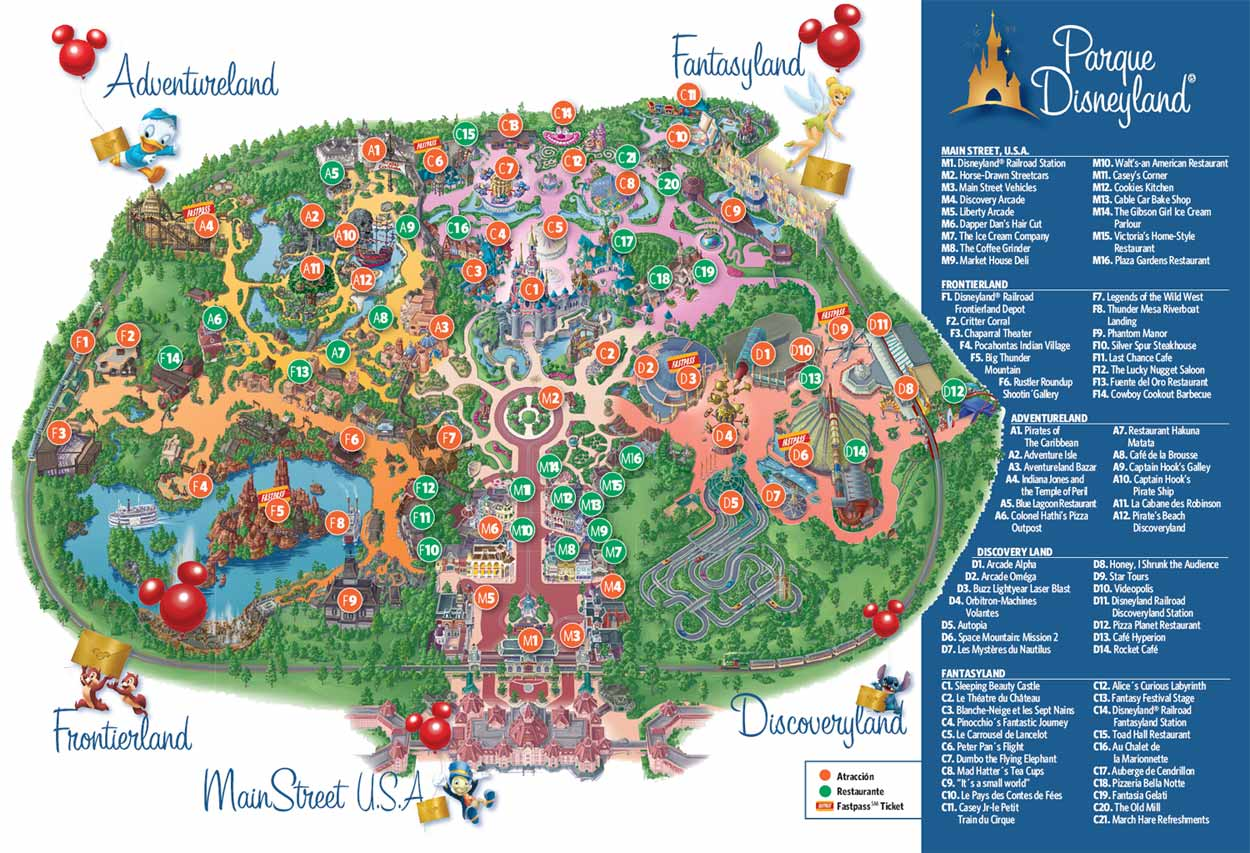
\includegraphics[width=0.75\textwidth]{imatges/mapa_disney_land_paris.jpg}\par\vspace{1cm}
    \caption{Mapa de \textit{Disney Land París}}
    \label{fig:disney1}
\end{figure}

\clearpage
\section{Objectiu}
L'objectiu del projecte és \textbf{fer la distribució dels restaurants més cars a partir d'unes determinades zones \say{remarcades} per maximitzar els beneficis del parc}. Aquestes zones les anomenarem candidates, i seran aquelles on es podran ubicar els restaurants.

Per aconseguir aquest objectiu es considerarà que el mapa d'atraccions del nou territori és el mateix que el de \textit{DLP}; que les \textit{Magic Bands} (\ref{fig:magic_bands}) recullen i emmagatzemen la informació de la posició dels seus usuaris cada 5 minuts, i que disposem de tantes zones candidates (o més) com restaurants es vulguin ubicar. 

Per determinar el grau d'interès de cada atracció, es compta amb una gran quantitat de dades generades per les \textit{Magic Bands} (\ref{fig:magic_bands}) que es reparteixen a l'entrada del parc temàtic, i que tenen per objectiu l'estudi del comportament del públic. 

\begin{figure}[H]
    \centering
    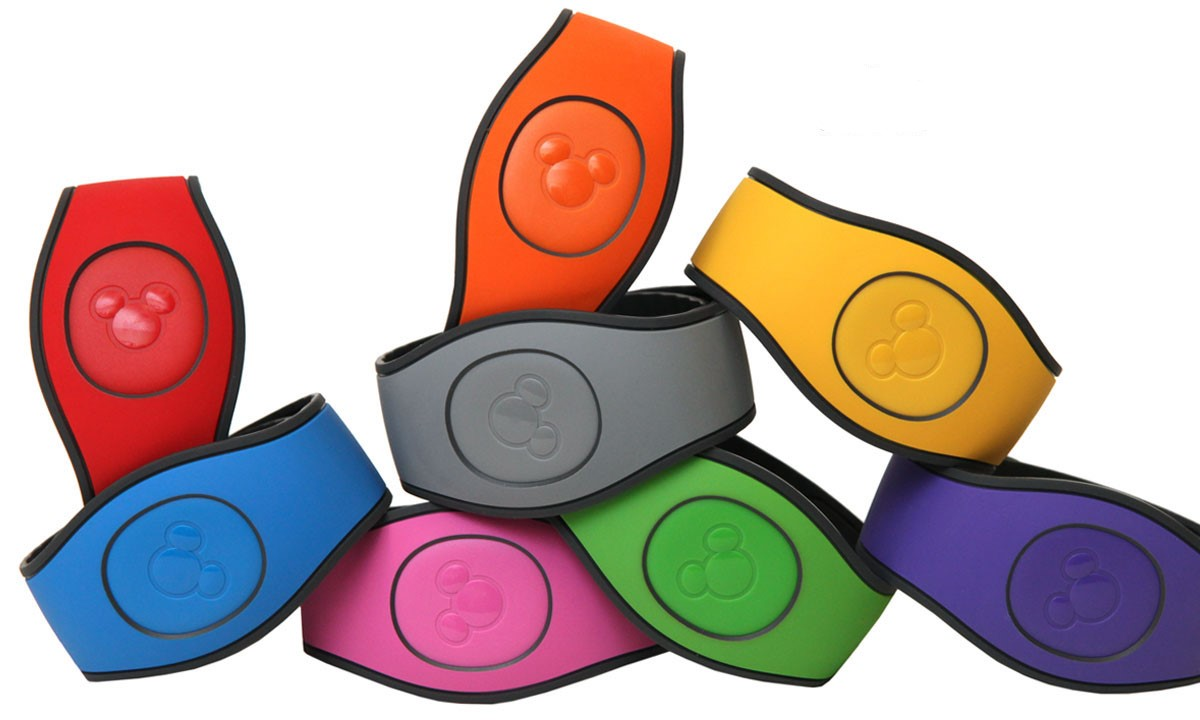
\includegraphics[width=0.75\textwidth]{imatges/magic_bands.jpg}\par\vspace{1cm}
    \caption{\textit{Magic Bands}}
    \label{fig:magic_bands}
\end{figure}

\clearpage
\section{Definició del problema}
Així doncs, per aconseguir l'objectiu que hem plantejat es seguiran 5 passos, que són:
\begin{enumerate}
	\item Assignar un pes a cada atracció.
	\item Dividir el mapa en àrees.
	\item Calcular la importància de cada atracció.
	\item Definir les zones candidates.
	\item Ubicar els restaurants.
\end{enumerate}

\subsection{Assignar un pes a cada atracció}
El pes d'una atracció es definirà a parir de la quantitat de gent que ha pujat a aquesta (aquesta informació es proporcionada per la direcció del parc). En la següent figura es pot veure el mapa amb el pes per a cada una de les atraccions.

\begin{figure}[H]
	\centering
	\includegraphics[width=0.6\textwidth]{imatges/pesos.png}\par\vspace{1cm}
	\caption{Pesos de cada atracció}
	\label{fig:mapa_areas}
\end{figure}

\subsection{Dividir el mapa en àrees \label{arees}}
A partir del pes de cada atracció (ubicat en l'entrada d'aquesta), es poden seguir diferents estratègies per calcular la regio de influència per cada una de les atraccions a partir del nombre de gent del voltant.

\subsubsection{Estratègies}
Algunes d'aquestes estratègies són:
\begin{itemize}
	\item Utilitzar un diagrama de \textit{voronoi} per definir la regió d'interès de cada atracció (cada persona dins d'aquesta àrea computa 1).
	\item Utilitzar l'estratègia del punt anterior, i per cada atracció, per cada una de les àreeas no definides pel pivot, computar les persones que hi ha com $\frac{1}{1+d}$ on $d$ correspon a la distància en metres des de la persona a l'entrada de l'atracció.
	\item Utilitzar la estratègia del punt anterior, però aquesta vegada comptant la distància ($d$) des de la persona al segment que defineix l'àrea regida pel pivot.
	\item Utilitzar diagrames de \textit{voronoi} de diferents nivells ($k$ on $2 \le k \le n$ i $n$ és el nombre d'atraccions), el diagrama de primer nivell defineix la regió de màxim interés de l'atracció (computant 1 per cada persona) i les $k-1$ \textbf{capes superposades} dels següents nivells, determinen zones d'interès però no tan importants (computen $\frac{1}{k}$ per cada persona).
\end{itemize}

\subsubsection{Diagrama de \textit{voronoi} de primer nivell}
Segons l'estratègia que es seguis, s'obtindria una distribució en àrees o un altre. En aquest cas s'ha obtat per utilitzar l'última proposta amb una $k = 2$, ja que es creu que és una bona aproximació pel problema que es vol resoldre. 

Abans però, cal fer la ubicació de ploígons que representin aquelles zones que un usuari no pot travessar en la seva ruta fins arribar a l'entrada de l'atracció, això evitarà obtenir dades poc realistes. En la següent figura es pot veure una possible representació del diagrama de \textit{voronoi} d'ordre 1.


\textbf{Falta posar els poligons que regeixen les zones prohibides, rius, llacs, les propies atraccions...}

\begin{figure}[H]
	\centering
	\includegraphics[width=1\textwidth]{imatges/diagrama_voronoi_ordre_1.png}\par\vspace{1cm}
	\caption{Diagrama de \textit{voronoi} d'ordre 1}.
	\label{fig:diagrama_voronoi_ordre_1}
\end{figure}

\subsubsection{Capa de \textit{voronoi} de segon nivell}
Per afinar més els càlculs, es vol calcular la capa superposada de \textit{voronoi} de segon nivell, i a partir d'aquesta obtenir una aproximació de la influència de les persones que estan pròximes a l'àrea definida en el primer nivell.


En la següent figura es pot veure el diagrama de \textit{voronoi} de segon nivell, el qual superposant-lo amb el diagrama de \textit{voronoi} de primer nivell, s'obtindria la capa de superposició que es vol.

\textbf{Falta posar els poligons que regeixen les zones prohibides, rius, llacs, les propies atraccions...}

\begin{figure}[H]
	\centering
	\includegraphics[width=1\textwidth]{imatges/diagrama_voronoi_ordre_1.png}\par\vspace{1cm}
	\caption{Diagrama de \textit{voronoi} d'ordre 2}.
	\label{fig:diagrama_voronoi_ordre_1}
\end{figure}

\subsection{Definir les zones candidates}
Un cop es disposa de la regió d'influència de cada atracció (veure Secció \ref{arees}). Es vol fer el posicionament dels restaurants, però abans cal que la direcció del parc proporcioni un mapa tot indicant quines són les possibles ubicacions per aquests restaurants. En la següent figura es mostren un possible mapa.

\begin{figure}[H]
	\centering
	\includegraphics[width=1\textwidth]{imatges/possibles_ubicacions.png}\par\vspace{1cm}
	\caption{Mapa amb les possibles ubicacions}.
	\label{fig:zones_candidates}
\end{figure}

\subsection{Ubicar els restaurants}
En aquest punt, la direcció ha de proporcionar una llista amb els restaurants que es volen ubicar amb un valor associat, aquest valor ha de reflexar quant car és cada restaurant.

Una vegada es tenen els restaurants a ubicar i les zones candidates, cal calcular el benefici de cada configuració a partir del benefici de cada restaurant i la influència que rep en base a les atraccions que té al voltant.  

Una vegada generada totes les combinacions, s'elegirà la que maximitzi el benefici global del parc. En la següent figura es mostra un exemple d'una possible solució.

\begin{figure}[H]
	\centering
	\includegraphics[width=0.9\textwidth]{imatges/solucio.png}\par\vspace{1cm}
	\caption{Mapa d'atraccions amb les ubicacions dels restaurants}.
	\label{fig:mapa_restaurants}
\end{figure}


\section{Pre-processament de dades}
Pel caràcter del problema i per evitar errors, es realitzarà un preprocessament amb els punts recollits, de tal manera que, només es consideraran els punts que:
\begin{itemize}
	\item S’han recollit dins d’un conjunt de franges horàries que es consideren d'interés pels visitants alhora de buscar un restaurant per anar a menjar. 
	Així doncs, el llistat de franges horàries a considerar és:
	\begin{itemize}
		\item Esmorzar: 9h-10h
		\item Dinar: 12h-14h
		\item Berenar: 17h-18h
		\item Sopar: 20h-22h
	\end{itemize}

	\item No s’hagin recollit a les zones on es troben obstacles. 
	Considerem obstacles a les atraccions, boscos, llacs….
\end{itemize}


%\subsection{Algoritme}

\clearpage
\section{Articles}

%\clearpage
%\section{Treball futur}

%\clearpage
%\section{Conclusions}

\clearpage
\begin{thebibliography}{9}
\bibitem{cert1}
Beneficis certificacions IT, 1.
\\\\\path{https://certification.comptia.org/es/por-qué-certificarse/profesionales}
\bibitem{cert2}
Beneficis certificacions IT, 2.
\\\\\path{https://certification.comptia.org/es/por-qu\%C3\%A9-certificarse}
\bibitem{cert3}
Beneficis certificacions IT, 3.
\\\\\path{https://www.microsoft.com/en-us/learning/certification-testimonials.aspx}
\end{thebibliography}
\end{document}
